\documentclass[../main.tex]{subfiles} % required, if the Chapter be a seperate doc

\begin{document}
\section{Zusammenfassende Tabellen}\label{sec:zusammenfassende-tabellen}
    \begin{figure}[H]
        \centering
        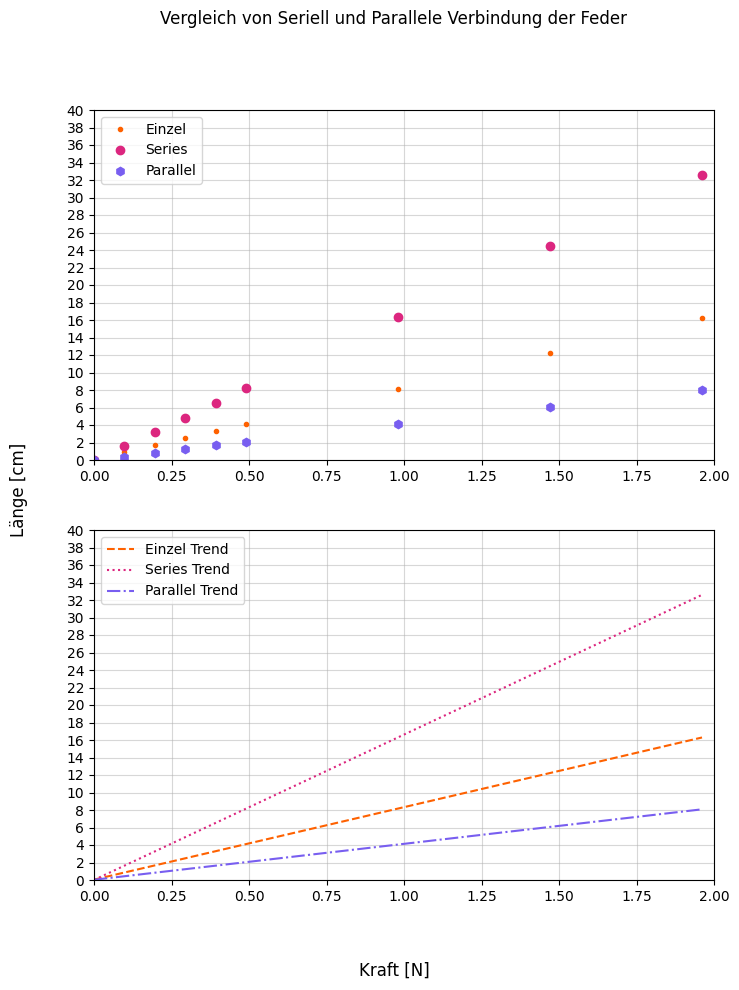
\includegraphics[scale=0.6]{graph/Spring-setup-comparison}
        \caption{Die Darstellung der Feder Positionen einzeln, in Seriell und in Parallel mit Datenpunkte und Trendlinien}\label{fig:figure}
    \end{figure}
    In der Tabelle kann man sehen, dass die parallele Konstellation mehr Kraft benötigt, \\
    um die gleiche Dehnung zu erreichen wie in der seriellen Konstellation.\\
    Wenn man die Federn in Serie schaltet, wird die Federkonstante halbiert.
    \section{Resultat}\label{subsec:resultat}
    Das Resultat unseres Experiments ist, dass die Feder konstante beider Federn 0.1209 N/cm beträgt.

\end{document}
